\documentclass[11pt]{article}
\usepackage[margin=1in]{geometry}
\usepackage{fancyhdr}
\usepackage{enumitem}
\usepackage{parskip}
\usepackage{xcolor}
\usepackage{graphicx}
\usepackage{amssymb}

% Personal notes: \comment{Write your thoughts here.}
% Notes appear in grey in the compiled document; blank lines are supported.
\definecolor{commentgray}{gray}{0.5}
\newcommand{\comment}[1]{{\color{commentgray}#1}}

\pagestyle{fancy}
\fancyhf{}
\fancyhead[C]{\textbf{CEG2136}}
\fancyfoot[C]{\thepage}

\newcounter{chapterNumber}
\setcounter{chapterNumber}{11}
\newcounter{headerOneCount}
\newcounter{headerTwoCount}[headerOneCount]
\setcounter{headerOneCount}{-1}
\renewcommand{\theheaderOneCount}{\arabic{headerOneCount}}
\renewcommand{\theheaderTwoCount}{\arabic{headerTwoCount}}

\newcommand{\Title}[1]{%
  \begin{center}
    \fontsize{24}{28}\selectfont\textbf{#1}
  \end{center}
  \vspace{1em}
}

\newcommand{\HeaderOne}[1]{%
  \refstepcounter{headerOneCount}%
  \setcounter{headerTwoCount}{-1}%
  \vspace{0.75em}
  \noindent\fontsize{18}{22}\selectfont\textbf{\arabic{chapterNumber}.\theheaderOneCount\ #1}\par
  \vspace{0.5em}
}

\newcommand{\HeaderTwo}[1]{%
  \refstepcounter{headerTwoCount}%
  \vspace{0.5em}
  \noindent\fontsize{16}{20}\selectfont\textbf{\arabic{chapterNumber}.\theheaderOneCount.\theheaderTwoCount\ #1}\par
  \vspace{0.4em}
}

\newcommand{\BodyText}[1]{%
  \fontsize{12}{15}\selectfont #1\par
}

\newenvironment{NumberedList}{%
  \begin{enumerate}[leftmargin=2em, itemsep=0.35em, topsep=0.35em]
}{%
  \end{enumerate}
}

\newenvironment{DottedList}{%
  \begin{itemize}[leftmargin=2em, itemsep=0.35em, topsep=0.35em, label=\textbullet]
}{%
  \end{itemize}
}

\begin{document}
\title{Instruction Cycle (EXEC) Memory-Reference Instructions (MRI)}

\textbf{EXAM QUESTION: Given a brand new instruction, tell me what should happen after fetch and decode.}
\begin{center}
  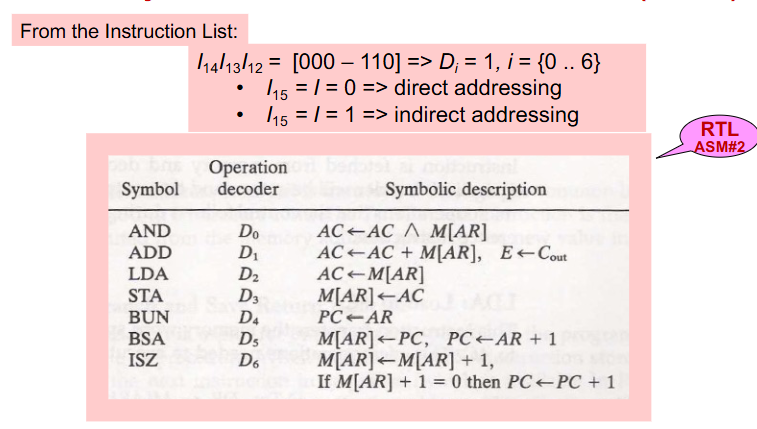
\includegraphics[width=1\textwidth]{11.1.png}
\end{center}

\begin{itemize}
  \item ADD is when $D_0$ which is decoder inputs $I_14$$I_13$$I_12$ = 000 
  \item so on for the rest
  \item The RTL/Symbolic Description is the desired micro-operation 
\end{itemize}

\subsection{Memory Reference Instructions}
\begin{itemize}
  \item \textbf{Starting point of command specific micro-ps for memory reference is at $T_4$. $T_0$ - $T_3$ is dedicated to fetch and decode.}
  \item \comment{Clarify with prof if its only memory reference and excludes cpu registers}
  \item \textbf{RTL notation is a abstracted version of the actual operations.}
\end{itemize}

\subsubsection{AND}

\begin{itemize}
  \item Operation Decode: $D_0$
  \item RTL Notation: AC $\leftarrow$ AC $\land$ M[AR] 
  \begin{itemize}
    \item AND to AC
    \item $D_0$$T_4$: DR $\leftarrow$ M[AR] Read operand 
    \item $D_0$$T_5$: AC $\leftarrow$ AC $\land$ DR, SC $\leftarrow$ 0 AND with AC, END program (SC $\leftarrow$ 0)
  \end{itemize}
\end{itemize}

\subsubsection{ADD}
\begin{itemize}
  \item Operation Decode: $D_1$
  \item RTL Notation: AC $\leftarrow$ AC $\land$ M[AR], E $\leftarrow$ $C_{out}$
  \begin{itemize}
    \item ADD to AC
    \item $D_1$$T_4$: DR $\leftarrow$ M[AR] Read operand 
    \item $D_1$$T_5$: AC $\leftarrow$ AC + DR, SC $\leftarrow$ 0, E $\leftarrow$ $C_{out}$
    \begin{itemize}
      \item E is the extend one-bit that is dedicated specifically to AC 
      \item Can also be used for signed and unsigned arithmetic. This includes shifting. 
    \end{itemize}
  \end{itemize}
\end{itemize}
    

\subsubsection{LDA}
\begin{itemize}
  \item Operation Decode: $D_2$
  \item RTL Notation: AC $\leftarrow$ AC $\land$ M[AR], E $\leftarrow$ $C_{out}$
  \begin{itemize}
    \item Load to AC
    \item $D_2$$T_4$: DR $\leftarrow$ M[AR] Read operand 
    \item $D_2$$T_5$: AC $\leftarrow$ DR, SC $\leftarrow$ 0 Store/Load DR in AC
  \end{itemize}
\end{itemize}

\subsubsection{LDA}
\begin{itemize}
  \item Operation Decode: $D_4$$T_4$ 
  \item RTL Notation: PC $\leftarrow$ AR, SC $\leftarrow$ 0 
  \item Moves curent PC value (Program count) to AR, SC reset meaning move onto next program. 
  \begin{itemize}
    \item \textbf{RECALL that a program counter points to each sequential command}
    \item branching unconditionally is essentially just asking PC to skip existing logic and go directly to a "line of code" 
\end{itemize}
  


    \item \comment{How does AR correlate to the correct PC skip}
    \item \textbf{Uses direct adressing (value at address) to set AR to be value we want PC to skip to.}
    \item \comment{Does the RTL not show the actual change to AR?}
    \item \textbf{No it doesnt.}
  \end{itemize}
  
  \item BSA
  \begin{itemize}
    \item Essentially, BUN with a way to return back to the original PC count.
    \item This is done by Storing the original PC count at AR, runs the subroutine at the new count. Once subroutine finishes call BUN back to the AR value (which contains the original count) 
  \end{itemize} 
  
  
  \item ISZ
  \subitem Operation Decode: $D_6$
  \begin{itemize}
    \item Increment and Skip-if-Zero
    \item $D_6$$T_4$ :DR $\leftarrow$ M[AR]
    \item $D_6$$T_5$ :DR $\leftarrow$ DR + 1 
    \item $D_6$$T_6$ :M[AR] $\leftarrow$ DR, if (DR = 0) then PC $\leftarrow$ PC + 1, SC $\leftarrow$ 0  
  \end{itemize}
  
  
\end{itemize}
  

\end{document}
